\section{User-Authentication}

\subsection{Registrieren eines neuen Nutzers}

Für die Registrierung eines neuen Nutzers müssen seine E-Mail-Adresse inklusive seines 
gewählten Passwords sowie seine Zustimmung zur an die API gesendet werden.\\
Dies geschieht über die Form im Signup-Screen.

\subsubsection{API-Routes}

Die benötigten API-Routen werden als statische Konstanten deklariert.
\begin{code}
    \centering
    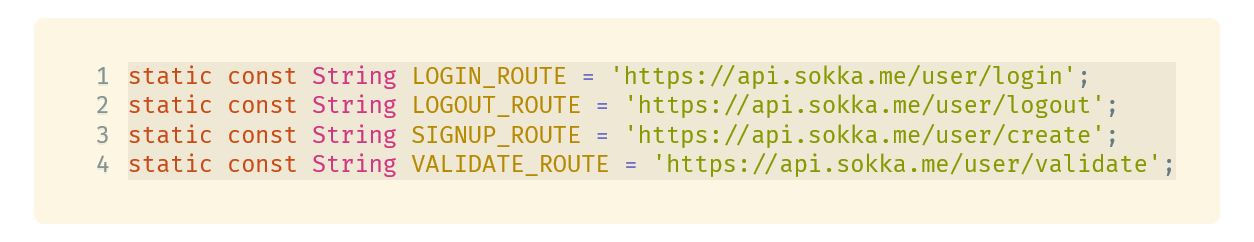
\includegraphics[width=1\textwidth]{images/Client/services/user-auth/userRoutes.png}
    \caption{Benötigte \lstinline{/user}-Routes der Sokka-API}
\end{code}

\begin{code}
    \centering
    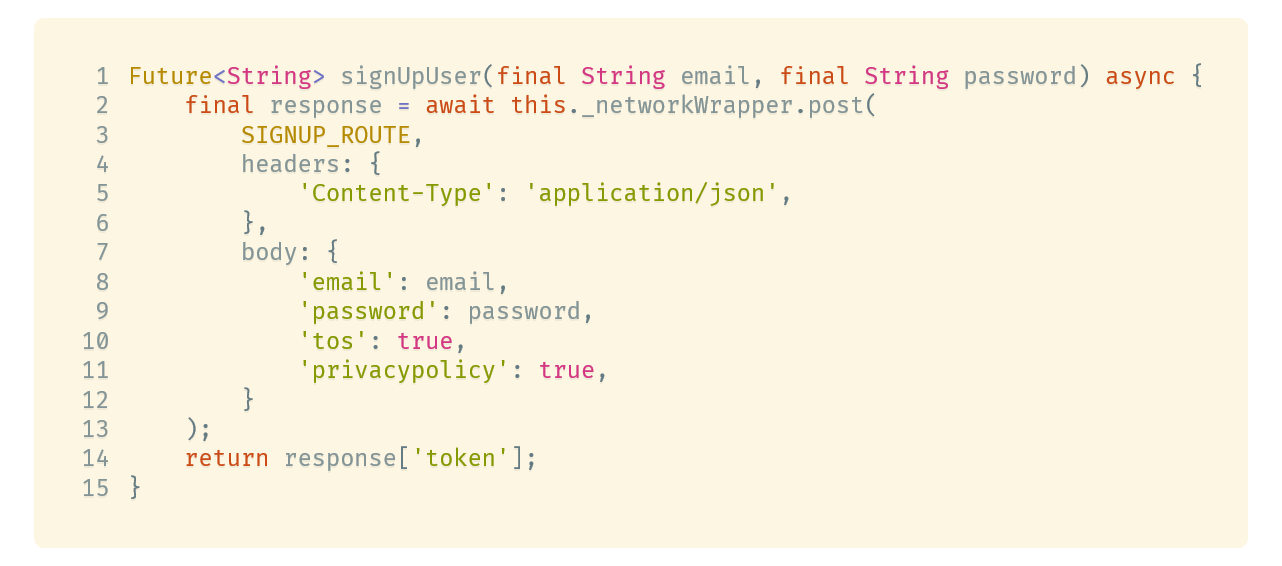
\includegraphics[width=1\textwidth]{images/Client/services/user-auth/signup.png}
    \caption{Funktion zum Registrieren eines neuen Nutzers}
\end{code}

\newpage

Ist der Request erfolgreich, so wird ein neuer Nutzer in der Datenbank erzeugt. Als Antwort wird der
Token für die damit generierte Nutzer-Session übermittelt, welcher in weiterer Folge im Cookie-Storage
abgespeichert wird.

\subsection{Anmelden eines vorhandenen Nutzers}

Zur Anmeldung eines bestehenden Nutzers in der App müssen dessen Logindaten an die 
\lstinline{/user/login}-Route der Sokka-API gesendet werden.\\
Gelingt der Request wird als Antwort der Token für die neu erzeugte Nutzer-Session gesendet.

\begin{code}
    \centering
    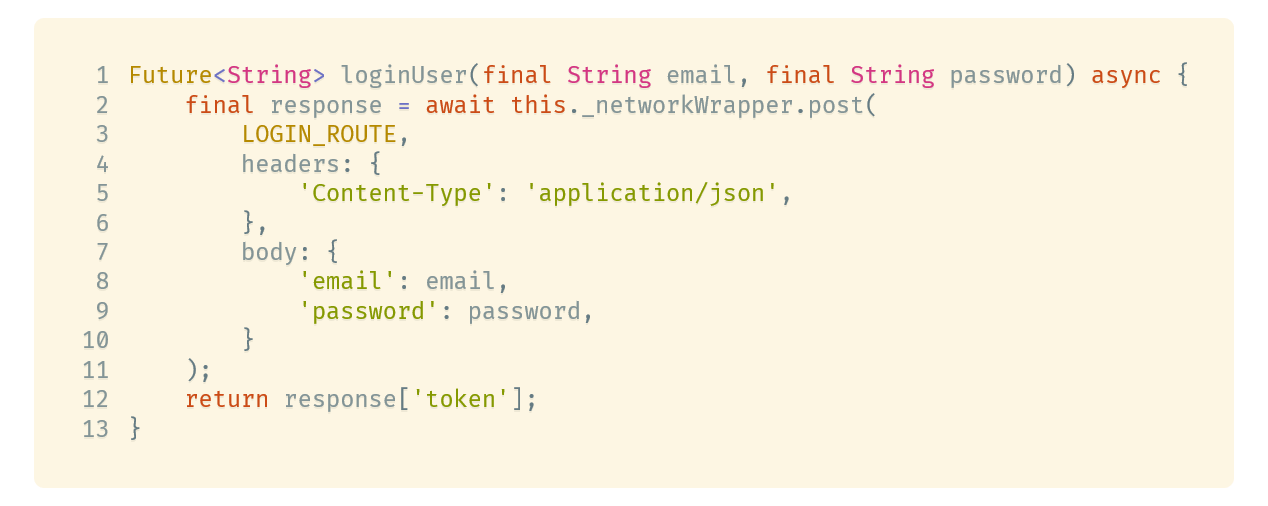
\includegraphics[width=1\textwidth]{images/Client/services/user-auth/login.png}
    \caption{Funktion zum Anmelden eines bestehenden Nutzers}
\end{code}

\subsection{Abmelden eines Nutzers}

Wenn sich ein Nutzers manuell in der App abmeldet wird ein Request an \lstinline{/user/logout} mit
dem gespeicherten Session-Token und der E-Mail des Nutzers gesendet.

Jener Session-Token wird in weiterer Folge ungültig gemacht und aus dem Cookie-Storage der App
gelöscht, wodruch der Nutzer beim nächsten App-Start wieder zum Login-Screen weitergeleitet wird.

\begin{code}
    \centering
    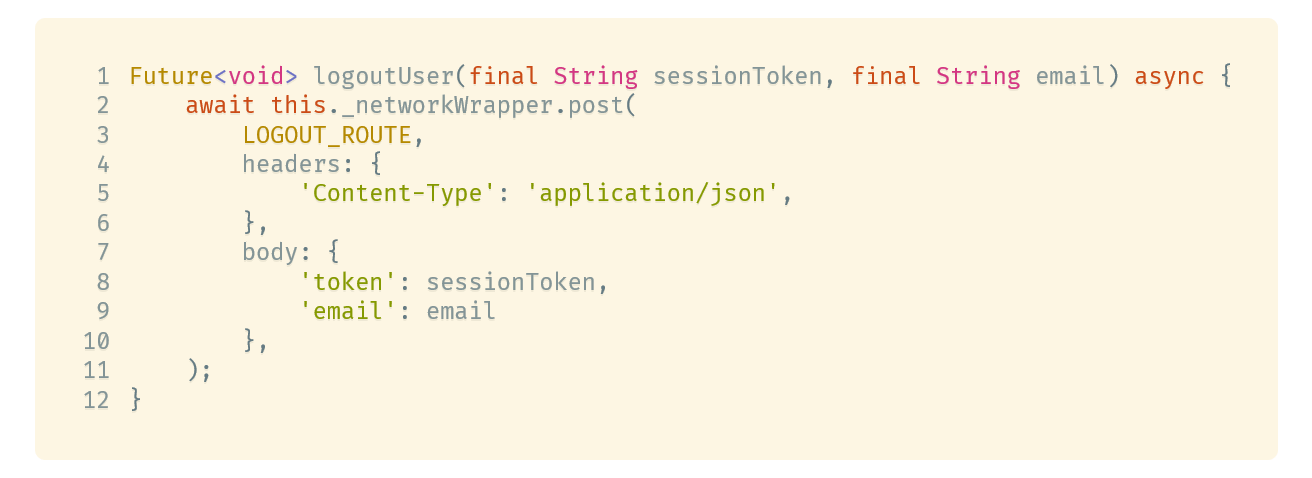
\includegraphics[width=1\textwidth]{images/Client/services/user-auth/logout.png}
    \caption{Funktion zum Abmelden eines Nutzers in der App}
\end{code}

\subsection{Validieren einer Nutzer-Session}

Damit sich ein Nutzer der Sokka-App nicht bei jedem Start der App mit seinen Logindaten neu
anmelden muss, werden die E-Mail-Adresse und der Session-Token nach einer erfolgreichen Anmeldung
im Cookie-Storage abgespeichert.

Mit jenen Daten im externen Gerätespeicher kann nun bei jedem weiteren App-Start ein Request an die
\lstinline{/user/validate}-Route mit Session-Token und E-Mail zur Validierung der Nutzer-Session
gesendet werden.\\
Wenn der Session-Token nachwievor gültig ist wird der Nutzer automatisch zum Home-Screen weitergeleitet.
Ist die Session abgelaufen erscheint der Login- bzw. Signup-Screen.

\begin{code}
    \centering
    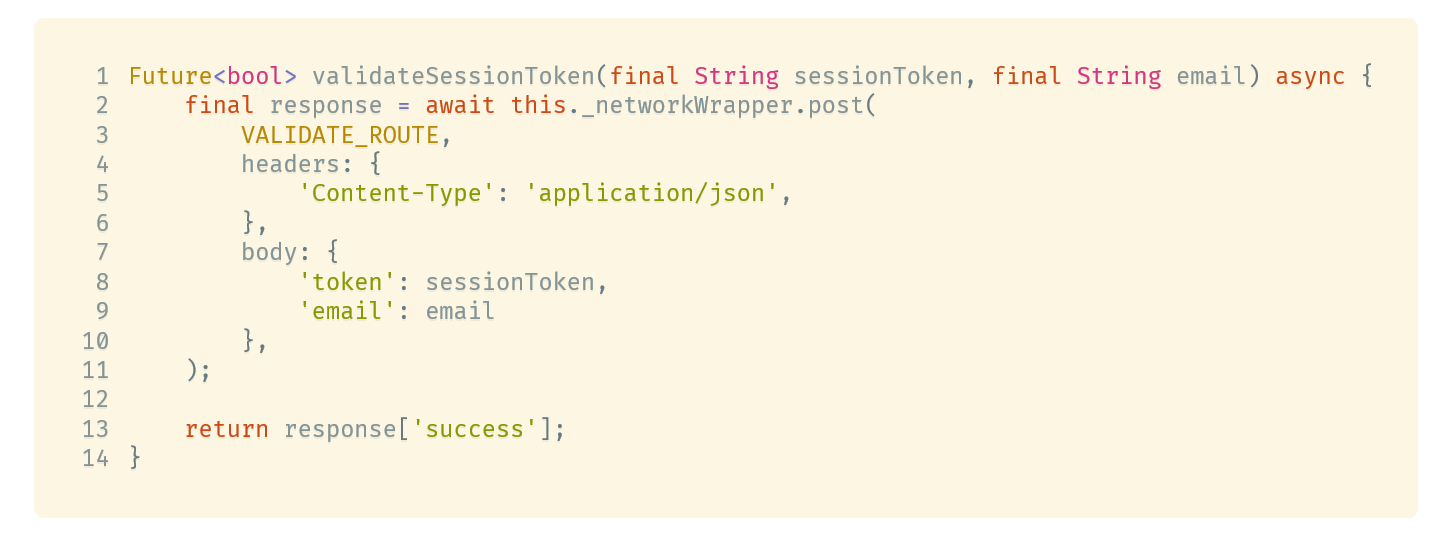
\includegraphics[width=1\textwidth]{images/Client/services/user-auth/validate.png}
    \caption{Funktion zur Validierung eines gespeicherten Nutzer-Session-Tokens}
\end{code}

\subsubsection{Wrapper-Funktion zur Session-Validierung}

Damit der Check der Validität des gespeicherten Session-Tokens einfach
bei Start der App ausgeführt werden kann gibt es folgende Wrapper-Funktion,
die automatisch benötigte Werte aus dem Storage nimmt und einen entsprechenden
Request an die Sokka-API sendet.

\begin{code}
    \centering
    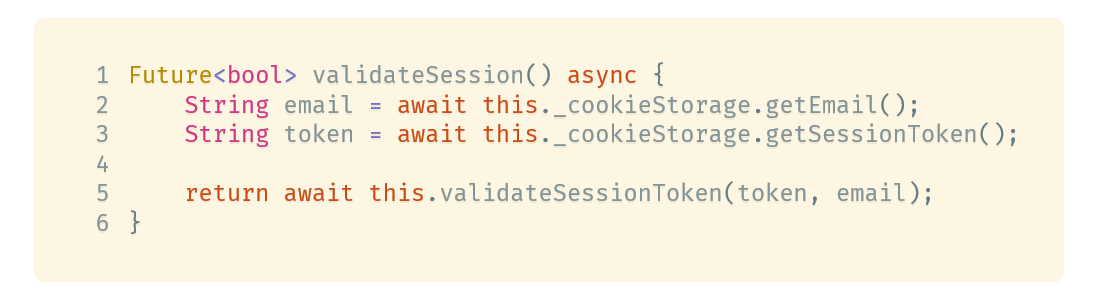
\includegraphics[width=1\textwidth]{images/Client/services/user-auth/validateSession.png}
    \caption{Wrapper-Funktion für die einfache Validierung eines Session-Tokens}
\end{code}